\documentclass[../main.tex]{subfiles}
\begin{document}
	\newpage
	\subsection{Sprint 2}
	
	\par Beim 2. Sprint hat sich das Team dem verbessern der User-Experience gewidmet.
	
	\begin{itemize}
		\item Steuerung mittels Tastatur ermöglichen
		\begin{itemize}
			\item Unity InputManager implementieren [5]
		\end{itemize}
		\item Spieler kann die Kamera bewegen
		\begin{itemize}	
			\item Bewegen der Kamera ermöglichen [3]
			\item Zoomen der Kamera ermöglichen [3]
		\end{itemize}
		\item Tilestack soll mit der Kamera bewegen
		\begin{itemize}
			\item Tilestack in den UI Layer verschieben [5]
			\item Tilestack UI überarbeiten [1]
		\end{itemize}
		\item Spiele soll einen Score haben
		\begin{itemize}
			\item Kalkulation eines \gls{score} implementieren [3]
			\item Score in der UI anzeigen [1]
		\end{itemize}
		\item Das Spiel soll Töne abspielen
		\begin{itemize}
			\item SoundManager implementieren [5]
			\item Platzieren eines Tiles soll einen Ton abspielen [2]
			\item Eruiere Musik/Töne zum abspielen [2]
		\end{itemize}
		\item Spiel soll eine Info-Sektion haben
		\begin{itemize}
			\item Hauptmenü soll ein Info-Popup erhalten [2]
		\end{itemize}
		\item Spiel soll ein Pasue-Menü haben
		\begin{itemize}
			\item Erlaube aus dem Spiel ins Hauptmenü zu kehren [2]
			\item Pausemenü erstellen [2]
			\item Pausemenü soll zurück ins Hauptmenü ermöglichen [1]
			\item Pausemenü soll auch das Info-Popup (Hauptmenü) enthalten [1]
			\item Im Spiel soll der Knopf "Zurück ins Hauptmenü" das Pausemenü öffnen [1]
		\end{itemize}
		\item Sprint 1 Review schreiben [2]
		\item Coding-Guidelines definieren [3]
	\end{itemize}

	\par Die Tasks wurden alle bis zum Sprintende fertig gestellt.
	
	\begin{figure}[H]
		\centering
		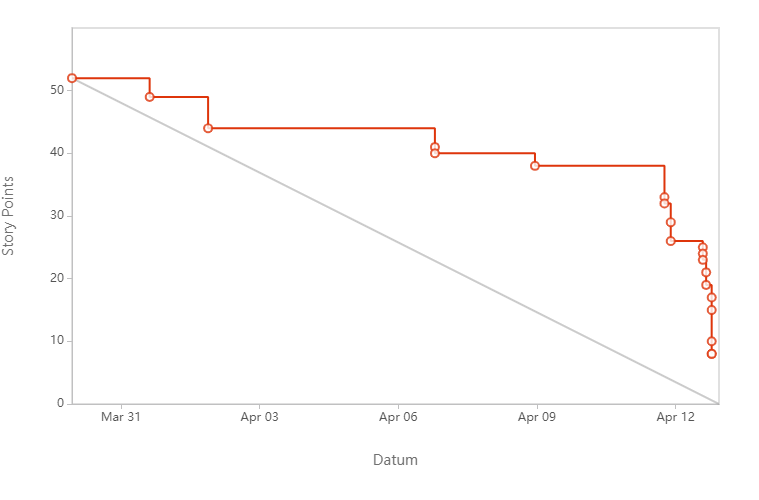
\includegraphics[width=0.5\textwidth]{Sprint_2_Burndown_Chart}
		\caption{Sprint 2 Burndown-Chart}
	\end{figure}

	\par Die Coding-Guidelines entsprechend mehrheitlich dem C\# Standard von Microsoft. Alle genutzten Regeln können \href{https://github.com/ktaranov/naming-convention/blob/master/C#Coding Standards and Naming Conventions.md}{hier} eingesehen werden.


\end{document}